\begin{exercise}
Analysiere den Beweis des Satzes über die offene Abbildung und zeige folgende
allgemeinere Variante: \\
Sei $X$ ein Banachraum, $Y$ ein normierter Raum und sei $A: X \rightarrow Y$ stetig
und linear und $A(X)$ sei von 2.Kategorie (für die Terminologie siehe Bemerkung
4.1.4 im Skriptum) in $Y$. Dann folgt:
\begin{enumerate}[label = (\roman*)]
  \item $A$ ist offen.
  \item $A(X) = Y$.
  \item $Y$ ist Banachraum.
\end{enumerate}
\end{exercise}
\begin{solution}
\begin{enumerate}[label = (\roman*)]
  \item
  Wir können $X = \bigcup_{k \in \N} U_k^X(0)$ schreiben. Es folgt
  \begin{align*}
    A(X) = A\left(\bigcup_{k \in \N} U_k^X(0)\right)
    = \bigcup_{k \in \N}A(U_k^X(0)).
  \end{align*}
  Die Voraussetzung $A(X)$ sei von 2.Kategorie besagt, dass sich $A(X)$
  nicht als abzählbare Vereinigung von nirgends dichten Mengen darstellen lässt.
  Es existiert also ein $k \in N: W := \overline{A(U_k^X(0))}^{\circ} \neq \emptyset$.
  Nun gilt, dass $W - W$ eine offene Nullumgebung ist und aufgrund der Stetigkeit
  der Addition ($+(\overline{A \times B}) \subseteq \overline{f(A \times B)}$)
  \begin{align*}
    W - W \subseteq \overline{A(U_k^X(0))} + \overline{A(U_k^X(0))}
    \subseteq \overline{A(U_k^X(0)) + A(U_k^X(0))}
    = \overline{A(U_k^X(0) + U_k^X(0))}
    = \overline{A(U_{2k}^X(0))}.
  \end{align*}
  Jetzt wähle $\epsilon > 0$, sodass
  \begin{align*}
    U_{\epsilon}^Y(0) \subseteq W - W \subseteq \overline{A(U_{2k}^X(0))}.
  \end{align*}
  Schließlich müssen wir unsere Abbildung $A$ noch skalieren:
  \begin{align*}
    B := \frac{2k}{\epsilon}A
  \end{align*}
  und es folgt aufgrund der Stetigkeit der Skalarmultiplikation
  \begin{align*}
    U_1^Y(0) = \frac{1}{\epsilon}U_{\epsilon}^Y(0) \subseteq
    \frac{1}{\epsilon} \overline{A(U_{2k}^X(0))}
    \subseteq \overline{A(U_{\frac{2k}{\epsilon}}^X(0))}
    = \overline{\frac{\epsilon}{2k}B(U_{\frac{2k}{\epsilon}}^X(0))}
    = \overline{B(U_{1}^X(0))}.
  \end{align*}
  Lemma 4.3.3 liefert uns dann sogar
  \begin{align*}
    U_1^Y(0) \subseteq B(U_{1}^X(0))
  \end{align*}
  und aufgrund Lemma 4.3.2 ist $B$ damit eine offene Abbildung. \\
  Sei nun $O \subseteq X$ eine beliebige offene Menge. Dann gilt
  \begin{align*}
    A(O) = \frac{\epsilon}{2k}B(O)
  \end{align*}
  ist offen, da $B(O)$ offen ist und die Skalarmultiplikation ein Homöomorphismus ist.
  Somit ist auch $A$ eine offene Abbildung.
  \item Wir wissen also, dass $A(X)$ offen und aufgrund der Linearität von $A$
  ein linearer Teilraum von $Y$ ist. Aus Aufgabe 3/2 wissen wir, dass
  jeder echter linearer Teilraum $X \subsetneq Y$ keinen inneren Punkt hat und
  daher nicht offen sein kann. Deswegen muss $A(X) = Y$ gelten-
  \item Die Abbildung $A$ stellt einen Homomorphismus zwischen den Vektorräumen
  $X$ und $Y$ dar. Definiere $N := \ker(A)$. Der Homomorphiesatz aus der Algebra
  sagt uns nun, dass es genau einen Homomorphismus $\varphi$ von der Faktormenge $A/N$
  nach $Y$ gibt mit
  \begin{align*}
    A = \varphi \circ \kappa,
  \end{align*}
  \begin{center}
  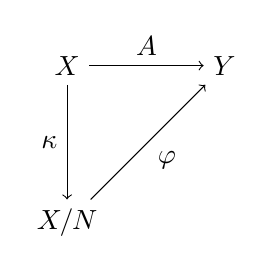
\begin{tikzpicture}[auto]
      \node (X) at (0,0) {$X$};
      \node (X/N) at (0,-2) {$X/N$};
      \node (Y) at (2,0) {$Y$};
      \draw[->] (X) to node  {$A$} (Y);
      \draw[->] (X) to node [swap]  {$\kappa$} (X/N);
      \draw[->] (X/N) to node [swap] {$\varphi$} (Y);
  \end{tikzpicture} \\
  \end{center}
  wobei $\kappa$ die kanonische Einbettung $A \rightarrow A/N$ darstellt.
  Mit Proposition 2.4.9 wissen wir außerdem, dass aus der Tatsache, dass $(X,||\cdot||)$
  ein Banachraum ist, bereits folgt, dass $(X/N, ||\cdot||_{X/N})$ ebenfalls ein
  Banachraum ist. $\varphi$ ist aufgrund der Surjektivität von $A$ sogar ein
  Isomorphismus. Wir zeigen schließlich noch, dass $\varphi$ ebenfalls eine offene Abbildung ist.
  Sei dazu $O \subset X/N$ offen. Dies ist genau dann der Fall, wenn
  \begin{align*}
     \widetilde{O} :=\bigcup_{[x]_\sim \in O} [x]_{\sim}
  \end{align*}
  in $X$ offen ist. Also gilt
  \begin{align*}
    \varphi(O) = \bigcup_{[x]_\sim \in O} \varphi([x]_{\sim})
    = \bigcup_{[x]_\sim \in O} \varphi \circ \kappa(x)
    = \bigcup_{[x]_\sim \in O} A(x)
    = A(\widetilde{O})
  \end{align*}
  ist offen und $\varphi$ eine offene Abbildung. Daraus folgt, dass $\varphi^{-1}$
  stetig ist und somit linear und beschränkt. Dies wiederum ist äquivalent zu
  \begin{align*}
    \exists a > 0: \forall [x]_\sim \in X/N: a||[x]_\sim|| \leq ||\varphi([x]_\sim)||.
  \end{align*}
  Damit sind alle Voraussetzungen für Lemma 4.3.6, angewandt auf $\varphi$ und $X/N$, erfüllt
  und es folgt schlussendlich, dass $Y$ ein Banachraum ist.
\end{enumerate}
\end{solution}
